\section{Auswertung}
\label{sec:Auswertung}
\subsection{Messung der Durchmesser der Löcher}

Zunächst wurde die Schallgeschwindigkeit in Acryl über das Zeitintervall $\increment t_1$ gemessen, welches den zeitlichen
Abstand zwischen der Aussendung eines Impulses und dessen Empfang wiedergibt. Dabei wurde die Weglänge zwischen der 
Oberseite des Acrylblocks und der Oberseite der Löcher $x_{\symup{A}}$ mithilfe einer Schieblehre ausgemessen.
\begin{figure}[H]
    \includegraphics{build/schall.pdf}
    \centering
    \caption{Zeit-Strecken Diagramm für die Schallwellen im Acrylblock.}
    \label{fig:schall}
\end{figure}
\noindent Dabei folgt der Graph der Gleichung
\begin{equation}
    x_{\symup{A}}=\symup{c}_{\symup{A}} \frac{\increment t_1}{2}-x_{\symup{M}}
    \label{eqn:gerade}
\end{equation}
wobei $x_{\symup{M}}$ die Distanz ist, die die Schallwelle in dem Messgerät selbst zurücklegt.
Aus Abbildung \ref{fig:schall} folgt dann für, dass $\symup{c}_{\symup{A}}=\qty{2862(91)}{\meter\per\second}$ und
$x_{\symup{M}}=\qty{5.2(1.3)}{\milli\meter}$ sind.\\
Zur Bestimmung der Durchmesser der Löcher wird dann die Zeit $\increment t_2$ vermessen, welche den Abstand zwischen
der Gegenüberliegenden Oberfläche zu der von $\increment t_1$ und den Löchern darstellt.
Die Durchmesser sind dann mit der Höhe des Blocks $\symup{h}$ über
\begin{equation}
    d=\symup{h}-x_{\symup{A}}-\symup{c} \increment t_2
    \label{eqn:durchmesser}
\end{equation}
bestimmt.
\begin{table}
  \captionsetup[table]{position=bottom} 
    \centering
    \label{tab:durchmesser}
    \sisetup{table-format=1.1, per-mode=reciprocal}
  \begin{tblr}{
    colspec = {S[table-format=2.1] S[table-format=1.1] S[table-format=1.1] S[table-format=3.2] S[table-format=3.2]},
      row{1} = {guard, mode=math},
      vline{2}={1}{-}{text=\clap{$\pm$}},
      vline{5}={4}{-}{text=\clap{$\pm$}},
  }
  \toprule
  d \text{/} \unit{\milli\meter} &   &d_{\symup{t}} \text{/} \unit{\milli\meter} &A \text{/} \unit{\percent} & \\
  \midrule
  14.9  & 3.5  &    7.7 &    93.20  &    45.36\\
   1.0  & 3.8  &    1.0 &     0.97  &   380.66\\
   7.9  & 3.7  &    1.0 &   692.13  &   364.68\\
   7.8  & 3.7  &    0.9 &   769.03  &   405.46\\
   7.9  & 3.7  &    1.1 &   620.13  &   331.53\\
   7.3  & 3.7  &    1.0 &   633.48  &   366.02\\
   8.8  & 3.6  &    1.8 &   387.78  &   201.52\\
   9.7  & 3.6  &    2.9 &   232.86  &   124.41\\
  11.1  & 3.6  &    4.0 &   177.82  &    89.38\\
   5.8  & 3.7  &    0.5 &  1057.85  &   739.39\\
   5.5  & 3.7  &    0.9 &   509.86  &   411.38\\
   \bottomrule
  \end{tblr}
  \caption{Die berechneten Durchmesser der Löcher $d$ mit ihren entsprechenden theoretischen Werten $d_{\symup{t}}$ 
und der Abweichung $A$ zwischen ihnen}
\end{table}



\subsection{Biometrische Untersuchung eines Augenmodells}

In Abbildung \ref{fig:Auge} ist der A-Scan des Augenmodells aufgeführt.
\begin{figure}
  \centering
  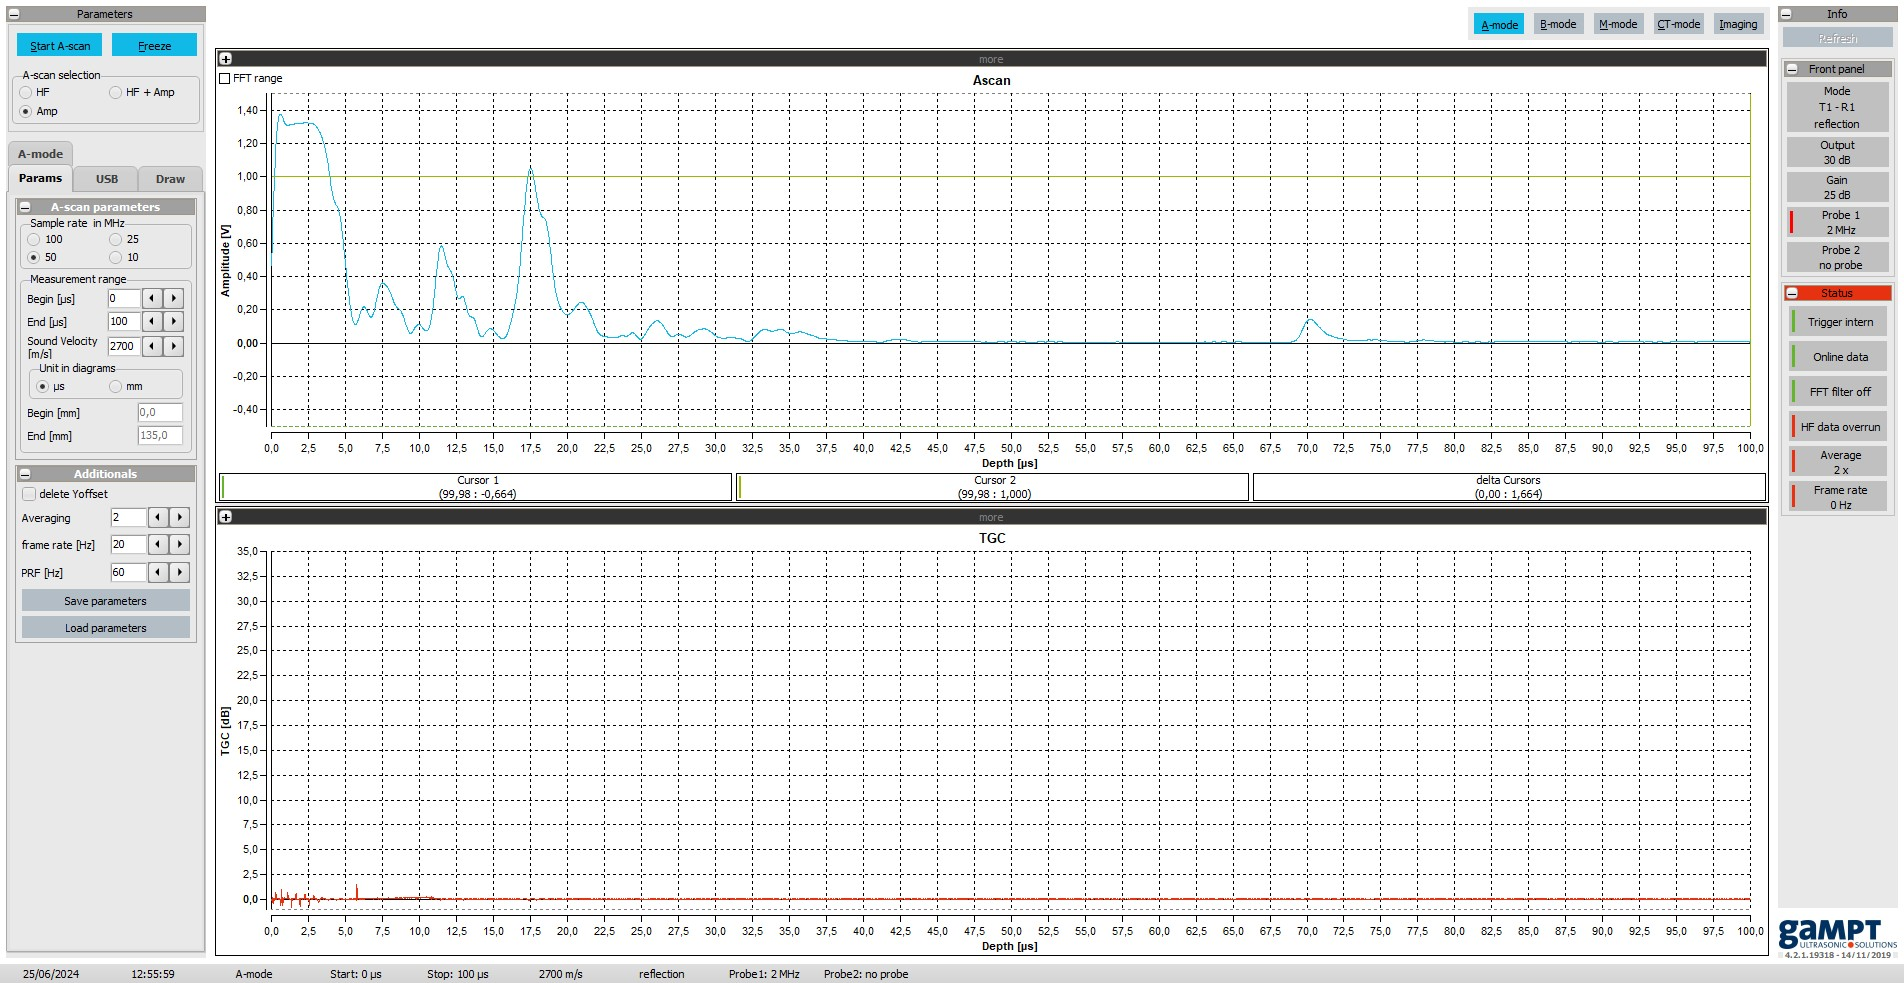
\includegraphics[width=\textwidth]{Bilder/Auge1.jpg}
  \caption{Abgebildet ist die Vermessung des Augenmodells mit dem A-Scan Verfahren}
  \label{fig:Auge}
\end{figure}

Die Zeiten, bei denen die Peaks auftreten, sind
\begin{gather*}
  t_{Iris}=   \qty{7.57}{\micro\second}\\
  t_{Linse_1}=\qty{11.56}{\micro\second}\\
  t_{Linse_2}=\qty{17.51}{\micro\second}\\
  t_{Retina}= \qty{70.17}{\micro\second} \, .
\end{gather*}

\noindent Zur Berechnung der Strecken wird von jedem dieser Werte $\frac{x_M}{c_A}$ abgezogen.
Mit der Schallgeschwindigkeit für die Glaskörperflüssigkeit $c_{GK}=\qty{1410}{\meter\per\second}$ lässt sich beim multiplizieren mit $t_{Iris}$ die Strecke bis zur Iris bestimmen.
Genau dasselbe wird für die Strecke zur Linse mit $t_{Linse_1}$ gemacht.
Danach muss für die Strecke in der Linse die Schallgeschwindigkeit $c_L=\qty{2500}{\meter\per\second}$ benutzt werden.
Bei dem Stück von dem Ende der Linse bis zur Retina wird wieder die Schallgeschwindigkeit der Glaskörperflüssigkeit verwendet.
Damit erbgeben sich die Werte
\begin{gather*}
  s_{Iris}=     \qty{8.1(0.6)}{\micro\second}\\
  s_{Linse_1}= \qty{13.7(0.6)}{\micro\second}\\
  s_{Linse_2}= \qty{28.6(0.6)}{\micro\second}\\
  s_{Retina}= \qty{102.9(0.6)}{\micro\second} \, .
\end{gather*}


\subsection{Untersuchung eines Brustmodells mit einem B-Scan}

In Abbildung \ref{fig:Brust} wird der B-Scan des Brustmodells dargestellt.
Durch grafische Auswertung wird dann die Breite von dem linken Tumor, mit $b_1=\qty{17.27}{\milli\meter}$ und die des rechten, mit $b_2=\qty{15.95}{\milli\meter}$, bestimmt.
Mit der Annahme, die Tumore seien Kugeln, wird deren Volumen ausgerechnet.
Es ergibt sich $V_1=\qty{234.25}{\milli\meter\cubed}$ und $V_2=\qty{199.81}{\milli\meter\cubed}$.
Zudem wird grafisch die Tiefe der Tumore, mit $d_1=\qty{17.11}{\milli\meter}$ und $d_2=\qty{11.39}{\milli\meter}$, gemessen.
Da Tumor 2 auf dem Bild vergleichsweise sehr hell erschein, handelt es sich bei diesem wahrscheinlich um einen, aus festem Gewebe bestehenden Tumor.
Bei Tumor 1 ist zu vermuten, dass es sich bei diesem um einen mit Flüssigkeit gefüllten Tumor, also um eine Zyste, handelt, da dieser weniger hell ist. 

\begin{figure}
  \centering
  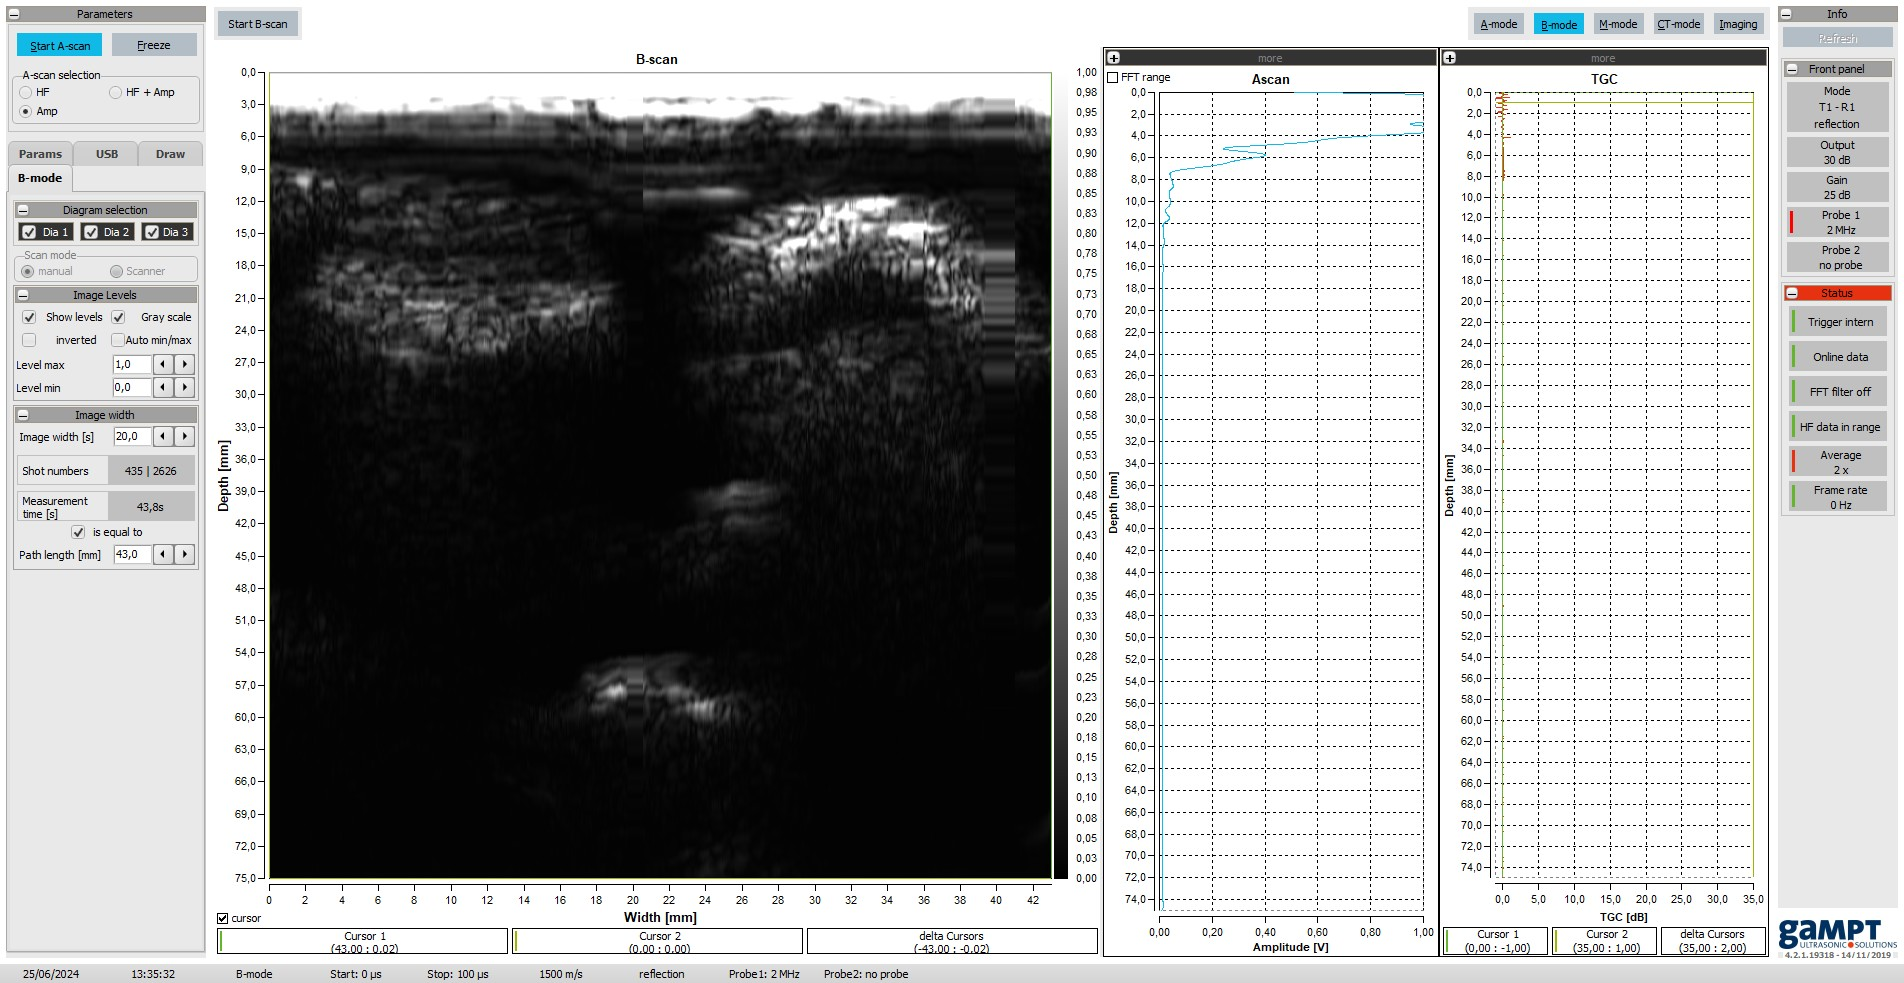
\includegraphics[width=\textwidth]{Bilder/Brust6.jpg}
  \caption{Hier ist Untersuchung des Brustmodells mithilfe des B-Scan Verfahrens aufgezeigt.}
  \label{fig:Brust}
\end{figure}

\subsection{Untersuchung eines Herzmodells mit einem TM-Scan}

Für die Untersuchung des Herzmodells wurden die Werte in Tabelle \ref{tab:Herz} aufgenommen.
Diese entsprechen einer grafischen Auswertung von Abbildung \ref{fig:Herz}.
$d$ ist dabei die gemessene Tiefe der Maxima unter dem Nullpunkt. 
Die Höhe der Peaks kann dann mit $h=\qty{75}{\milli\meter}-d-h_0$ bestimmt werden, wobei $h_0=44.21$ der gemessenen Baseline entspricht.

\begin{figure}[H]
  \centering
  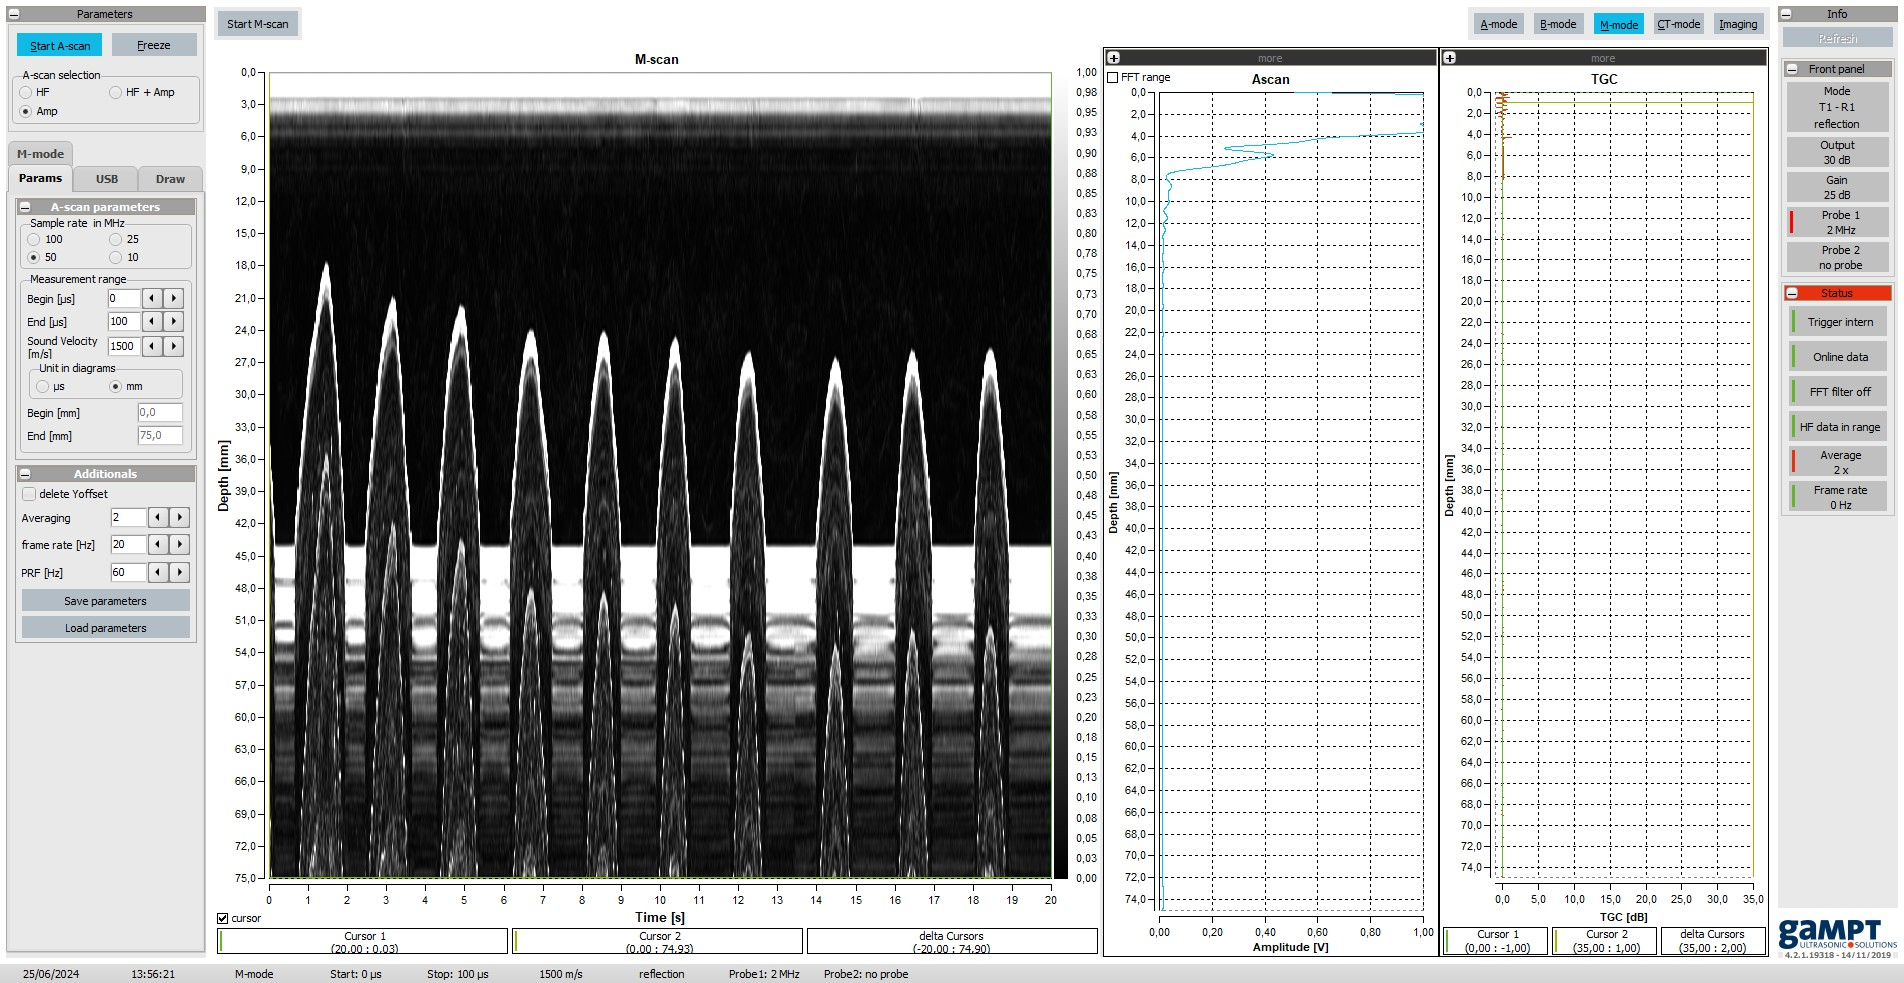
\includegraphics[width=\textwidth]{Bilder/Herz.jpg}
  \caption{Abgebildet ist ein TM-Scan eines Herz-Modells.}
  \label{fig:Herz}
\end{figure}


\begin{table}[H]
  \centering
  \label{tab:Herz}
  \sisetup{table-format=1.1, per-mode=reciprocal}
  \begin{tblr}{
      colspec = {S[table-format=3.0] S[table-format=2.1] S},
      row{1} = {guard, mode=math},
    }
    \toprule
    d \mathbin{/} \unit{\milli\meter} & T \mathbin{/} \unit{\second}  \\
    \midrule
    17.85 &  1.33\\
    21.03 &  1.12\\
    21.75 &  1.02\\
    24.03 &  1.03\\
    24.12 &  1.97\\
    24.57 &  0.87\\
    26.11 &  0.93\\
    26.66 &  0.95\\
    25.93 &  0.95\\
    25.75 &  0.86\\
    \bottomrule
  \end{tblr}
  \caption{Höhe und Breite der Peaks beim TM-Scan des Herzmodells.}
\end{table}

Das endsystolische Herzvolumen (ESV) kann hier als Kegelvolumen berechnet werden, wobei die Höhe des Peaks der Höhe des Kegels entspricht und die Grundfläche der Fläche des Herzmodells.
Dabei wird die Höhe über alle gemessenen Höhen gemittelt.
Das Volumen des Kegels kann mit 
\begin{equation}
  V=\frac{1}{3}\cdot \pi r^2 \cdot h 
  \label{eqn:Volumen}
\end{equation}
berechnet werden.
Der Durchmesser des Herzmodelles ist $\qty{43.7}{\milli\meter}$.
Es ergibt sich eine Höhe von $\bar{h}=\qty{7.0(2.6)}{\milli\meter}$ und damit das Volumen $\symup{ESV}=\qty{3.5(1.3)e3}{\milli\meter\cubed}$.
Die Herzfrequenz ergibt sich aus dem Inversen der gemittelten Periodendauer $T$.
Diese ist damit $\nu_{Herz}=\qty{0.91(0.26)}{\hertz}$.
Mit der Formel
\begin{equation}
  \symup{HZV}=(\symup{ESV}-\symup{EDV}) \cdot \nu_{Herz}
  \label{eqn:Herz}
\end{equation}
wird dann das Herzzeitvolumen bestimmt.
Das endiastolische Volumen (EDV) ist bei dem Modell 0.
Damit ergibt sich $\symup{HZV}=\qty{3.2(1.5)e3}{\milli\meter\cubed\per\second}$.
Umgerechnet ist das $\symup{HZV}=\qty{0.19(0.09)}{liter\per\minute}$.
